\documentclass{article}
\usepackage{sidecap}
\usepackage{float}
\usepackage[utf8]{inputenc}
\usepackage{graphicx}
\usepackage{mathtools,amsmath,amssymb} % Math packages
\usepackage{lipsum}
\usepackage[table]{xcolor}

% Font Package
\usepackage{lmodern}
\usepackage[T1]{fontenc}
\usepackage{textcomp}
\usepackage{booktabs}
\usepackage{tikz}
%\usepackage{natbib} % package for bibliography and citation

\usepackage{pdfpages}

\usepackage{subfiles} % Best loaded last in the preamble
%%%%%%%%%%%%%%%%%%%%%%%%%%%%%%%%%%%%%%%%%%%%%%%%%%%%%%%%%
%% R code packages


% Options for packages loaded elsewhere
\PassOptionsToPackage{unicode}{hyperref}
\PassOptionsToPackage{hyphens}{url}
%

\usepackage{lmodern}
\usepackage{amssymb,amsmath}
\usepackage{ifxetex,ifluatex}
\ifnum 0\ifxetex 1\fi\ifluatex 1\fi=0 % if pdftex
  \usepackage[T1]{fontenc}
  \usepackage[utf8]{inputenc}
  \usepackage{textcomp} % provide euro and other symbols
\else % if luatex or xetex
  \usepackage{unicode-math}
  \defaultfontfeatures{Scale=MatchLowercase}
  \defaultfontfeatures[\rmfamily]{Ligatures=TeX,Scale=1}
\fi
% Use upquote if available, for straight quotes in verbatim environments
\IfFileExists{upquote.sty}{\usepackage{upquote}}{}
\IfFileExists{microtype.sty}{% use microtype if available
  \usepackage[]{microtype}
  \UseMicrotypeSet[protrusion]{basicmath} % disable protrusion for tt fonts
}{}
\makeatletter
\@ifundefined{KOMAClassName}{% if non-KOMA class
  \IfFileExists{parskip.sty}{%
    \usepackage{parskip}
  }{% else
    \setlength{\parindent}{0pt}
    \setlength{\parskip}{6pt plus 2pt minus 1pt}}
}{% if KOMA class
  \KOMAoptions{parskip=half}}
\makeatother
\usepackage{xcolor}
\IfFileExists{xurl.sty}{\usepackage{xurl}}{} % add URL line breaks if available
\IfFileExists{bookmark.sty}{\usepackage{bookmark}}{\usepackage{hyperref}}
\hypersetup{
  hidelinks,
  pdfcreator={LaTeX via pandoc}}
\urlstyle{same} % disable monospaced font for URLs
%\usepackage[margin=1in]{geometry}
\usepackage{color}
\usepackage{fancyvrb}
\newcommand{\VerbBar}{|}
\newcommand{\VERB}{\Verb[commandchars=\\\{\}]}
\DefineVerbatimEnvironment{Highlighting}{Verbatim}{commandchars=\\\{\}}
% Add ',fontsize=\small' for more characters per line
\usepackage{framed}
\definecolor{shadecolor}{RGB}{248,248,248}
\newenvironment{Shaded}{\begin{snugshade}}{\end{snugshade}}
\newcommand{\AlertTok}[1]{\textcolor[rgb]{0.94,0.16,0.16}{#1}}
\newcommand{\AnnotationTok}[1]{\textcolor[rgb]{0.56,0.35,0.01}{\textbf{\textit{#1}}}}
\newcommand{\AttributeTok}[1]{\textcolor[rgb]{0.77,0.63,0.00}{#1}}
\newcommand{\BaseNTok}[1]{\textcolor[rgb]{0.00,0.00,0.81}{#1}}
\newcommand{\BuiltInTok}[1]{#1}
\newcommand{\CharTok}[1]{\textcolor[rgb]{0.31,0.60,0.02}{#1}}
\newcommand{\CommentTok}[1]{\textcolor[rgb]{0.56,0.35,0.01}{\textit{#1}}}
\newcommand{\CommentVarTok}[1]{\textcolor[rgb]{0.56,0.35,0.01}{\textbf{\textit{#1}}}}
\newcommand{\ConstantTok}[1]{\textcolor[rgb]{0.00,0.00,0.00}{#1}}
\newcommand{\ControlFlowTok}[1]{\textcolor[rgb]{0.13,0.29,0.53}{\textbf{#1}}}
\newcommand{\DataTypeTok}[1]{\textcolor[rgb]{0.13,0.29,0.53}{#1}}
\newcommand{\DecValTok}[1]{\textcolor[rgb]{0.00,0.00,0.81}{#1}}
\newcommand{\DocumentationTok}[1]{\textcolor[rgb]{0.56,0.35,0.01}{\textbf{\textit{#1}}}}
\newcommand{\ErrorTok}[1]{\textcolor[rgb]{0.64,0.00,0.00}{\textbf{#1}}}
\newcommand{\ExtensionTok}[1]{#1}
\newcommand{\FloatTok}[1]{\textcolor[rgb]{0.00,0.00,0.81}{#1}}
\newcommand{\FunctionTok}[1]{\textcolor[rgb]{0.00,0.00,0.00}{#1}}
\newcommand{\ImportTok}[1]{#1}
\newcommand{\InformationTok}[1]{\textcolor[rgb]{0.56,0.35,0.01}{\textbf{\textit{#1}}}}
\newcommand{\KeywordTok}[1]{\textcolor[rgb]{0.13,0.29,0.53}{\textbf{#1}}}
\newcommand{\NormalTok}[1]{#1}
\newcommand{\OperatorTok}[1]{\textcolor[rgb]{0.81,0.36,0.00}{\textbf{#1}}}
\newcommand{\OtherTok}[1]{\textcolor[rgb]{0.56,0.35,0.01}{#1}}
\newcommand{\PreprocessorTok}[1]{\textcolor[rgb]{0.56,0.35,0.01}{\textit{#1}}}
\newcommand{\RegionMarkerTok}[1]{#1}
\newcommand{\SpecialCharTok}[1]{\textcolor[rgb]{0.00,0.00,0.00}{#1}}
\newcommand{\SpecialStringTok}[1]{\textcolor[rgb]{0.31,0.60,0.02}{#1}}
\newcommand{\StringTok}[1]{\textcolor[rgb]{0.31,0.60,0.02}{#1}}
\newcommand{\VariableTok}[1]{\textcolor[rgb]{0.00,0.00,0.00}{#1}}
\newcommand{\VerbatimStringTok}[1]{\textcolor[rgb]{0.31,0.60,0.02}{#1}}
\newcommand{\WarningTok}[1]{\textcolor[rgb]{0.56,0.35,0.01}{\textbf{\textit{#1}}}}
\usepackage{graphicx,grffile}
\makeatletter
\def\maxwidth{\ifdim\Gin@nat@width>\linewidth\linewidth\else\Gin@nat@width\fi}
\def\maxheight{\ifdim\Gin@nat@height>\textheight\textheight\else\Gin@nat@height\fi}
\makeatother
% Scale images if necessary, so that they will not overflow the page
% margins by default, and it is still possible to overwrite the defaults
% using explicit options in \includegraphics[width, height, ...]{}
%\setkeys{Gin}{width=\maxwidth,height=\maxheight,keepaspectratio}
% Set default figure placement to htbp
%\makeatletter
%\def\fps@figure{htbp}
\makeatother
\setlength{\emergencystretch}{3em} % prevent overfull lines
\providecommand{\tightlist}{%
  \setlength{\itemsep}{0pt}\setlength{\parskip}{0pt}}
\setcounter{secnumdepth}{-\maxdimen} % remove section numbering

%%%%%%%%%%%%%%%%%%%%%%%%%%%%%%%%%%%%%%%%%%%%%%%%%%%%%%%%%%
\usepackage[margin = 1in, top = 0.8in, bottom = 0.8in]{geometry}
\title{Final Project: Analysis of Wine Quality Data}
\author{Robert West, Amirreza Sahebi Fakhrabad, Mohsen Sahraei Ardakani, Qiaozhi Bao,  \\Nasrin Alizadeh}
\date{November 2020}

\begin{document}

\maketitle

\section*{Executive Summary}
Identifying any relation between the chemical components of the wine and its desirability can be interest for wine companies. In this project we analyse the red wine data consisting of several chemical properties of wine and quality ratings to shed light on this question. The data contains observations on the chemical components of red wine from the Vinho Verde region in Portugal. \\
For the first step, our team did some preprocessing analysis to prepare the data for the different regression and classification methods. For this purpose, we checked the normality of the variables and also detected the outliers to improve the performance of the methods. The team decided to more focus on investigating classification methods since the target variable is an ordinal variable and contains the rates from $1$ to $10$ by tasters. We considered a variety of models including: logistic regression, LDA and QDA, KNN method, tree based methods and SVM. The models were compared with another based on the test errors.  \\Random Forest has the best average accuracy on test set with $19.4\%$ error, but bagging works competitively close and in some cases better. SVM and Boosting are other competitive algorithms. The team also figured out some variables such as "residual.sugar", "citric.acid", "fixed acidity" and "chlorides" do not play a significant role in the quality of the wine. On the other side, "alcohol", "sulphates", and "volatile.acidity" are the most significant factors effecting the ratings.

\section{1  Introduction}
The quality of wine and capturing the satisfaction of the customers can raise the question if there is any chemical factors influencing the quality of wine from customers' view of point. Our team explore red wine data to answer this question and determine the significant factors to classify the high quality wine. \\In the following, we first present the analyse conducted to preprocess the data. Then, the methods are provided with the detailed results. In the results section we compare the methods according to their test errors. And finally, we have the conclusion and appendix.

\subsection{1.1  Data}

Data is collected on 12 different variables and consisted of 1599 observations. The properties of wine that are measured are: fixed acidity, volatile acidity, citric acid, residual sugar, chlorides, free sulfur dioxide, total sulfur dioxide, density, pH, sulphates, alcohol and output variable (based on sensory data) quality (score between 1 and 10). All these properties are continuous but not quality, which is categorical variable.

As a part of the data pre-processing for statistical analysis, the team performed several exploratory analysis on the dataset. The dataset has no missing data. Furthermore, we provided the correlation between all the properties in Figure1. There is a high correlation between  "fixed.acidity" with "pH", "density" and "citric.acid".
That is why our team decided to perform lasso to explore the possibility of removing some of the variables.

After implementing Lasso we decided to keep "volatile.acidity", "chlorides", "pH", "sulphates" and "alcohol" and created a new variable "ratio\_sulfor.dioxide" which is ratio of free and total sulfor dioxide. 

\begin{figure}[H]
\begin{minipage}[]{.4\textwidth}
    \centering
    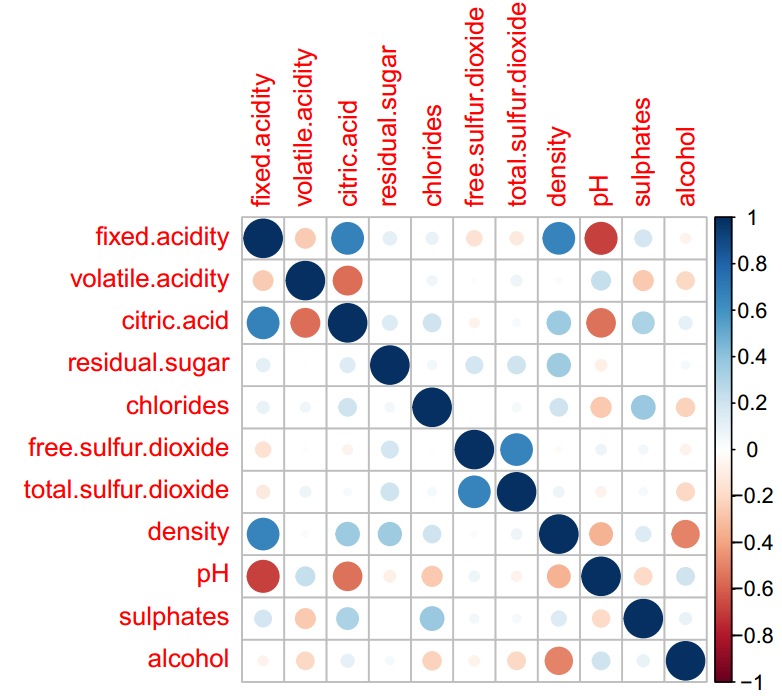
\includegraphics[scale=0.5]{Correlation.PNG}
    \caption{Correlation}
    \label{fig:Cor}
\end{minipage}
\hspace{0.5cm}
\begin{minipage}[]{.6\textwidth}
    \centering
    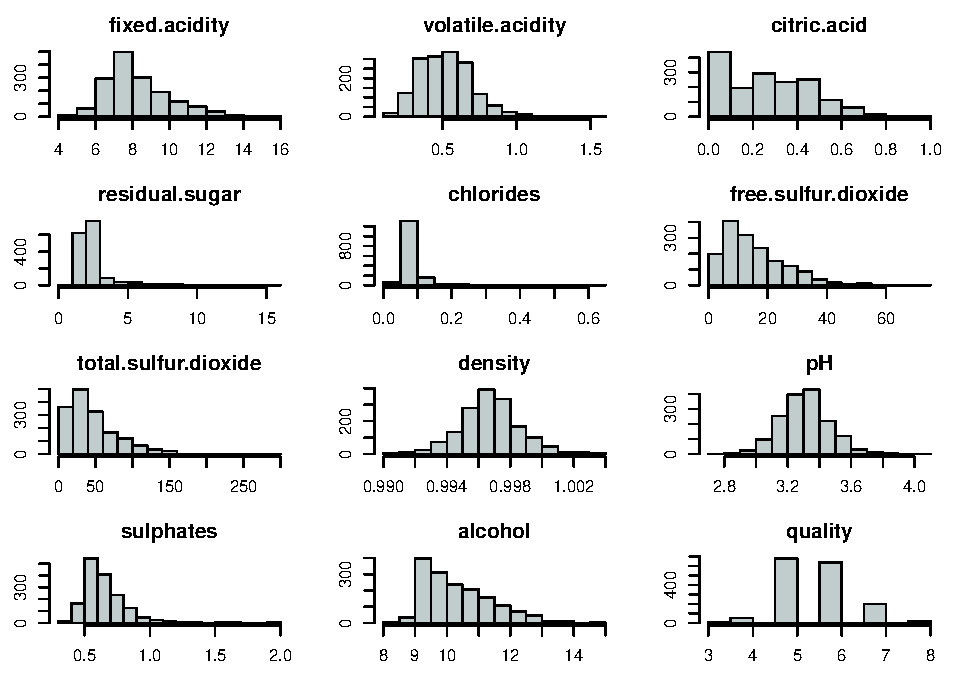
\includegraphics[scale=0.6]{Hist.pdf}
    \caption{Histogram}
    \label{fig:Hist}
\end{minipage}
\end{figure}




We also checked Normality of the predictors which is an assumption for methods like LDA and QDA. The easiest way to check normality is looking at the histograms of variables. As shown in figure \eqref{fig:Hist}, "chlorides", "sulphates" and "alcohol" have distributions far from Normal. So we implement some transformations to make them more close to Normal. (We just checked selected variables from lasso because LDA and DQA are the only models require Normality along with variable selection). Specifically, $log_{10}$, is used for "alcohol" and "sulphates", and square root is used for "alcohol".

Detecting and removing outliers is the last  step in our data cleaning process. We found outliers by looking at each selected variable's histogram and in total 37 observations are removed. We put the detailed analysis in the Appendix.

Note that some not all methods require variable selection, outlier detection or normality transformation. Thus we use them as needed. 

Regarding the response "quality", we decided to redefine it as two-level factor. For this new qualitative response, classes 3,4,5 are labeled as "Low" and classes 6,7,8 are labeled as "High" quality. We also explored other splits with more than two classes, and different two level ones. However, the best performance achieved in the split we chose. We could also use original quality levels as 6 separated classes, but there were some drawbacks: 1) Some levels (like 3 and 4) have small number of observations so their test error were not reliable 2) Some methods like QDA does not work properly when classes have small number of observations 3) Logistic Regression requires two classes. 
\section{2  Methods}
In this section, the methods including: logistic regression, LDA, QDA, KNN, decision tree, random forest, bagging, boosting and SVM are presented in detail. For each method, we report the related figures and analysis.
\subsection{2.1  Logistic Regression}
Logistic Regression is a productive classification technique to allow us predict a qualitative response. In this section, we use the predictors selected by lasso analysis,then look for the best model. The performance of the optimal model evaluated with accuracy and test error rates.
The team investigated six different models,using cross validation method to get accuracy measurement which describes how well each model works on the training set.Our candidate models are as follows:\\
\begin{table}[]
    \centering
    \begin{tabular}{|p{3cm}|p{11cm}|}
    \hline
        \textbf{Model 1} & $qualityBinary \sim volatile.acidity+chlorides+pH+sulphates + alcohol+ratio\_sulfur.dioxide$ \\
        
         \hline
         \textbf{Model 2}& $qualityBinary \sim volatile.acidity+chlorides+pH +sulphates + I(sulphates^2)+ I(sulphates^3)+alcohol+ratio\_sulfur.dioxide$ \\
         \hline
         \textbf{Model 3}&  $qualityBinary \sim chlorides+pH +sulphates + I(sulphates^2)+ I(sulphates^3)+alcohol+ratio\_sulfur.dioxide+I(ratio\_sulfur.dioxide^2)$\\
         \hline
         \textbf{Model 4}& $qualityBinary \sim chlorides*pH +chlorides*sulphates+chlorides*alcohol+ratio\_sulfur.dioxide$ \\
         \hline
         \textbf{Model 5}&  $qualityBinary \sim volatile.acidity+pH +sulphates + I(sulphates^2)+ I(sulphates^3)+alcohol+ratio\_sulfur.dioxide$\\
         \hline
         \textbf{Model 6}&  $qualityBinary \sim volatile.acidity+chlorides+pH +sulphates + I(sulphates^2)+ I(sulphates^3)+alcohol+ratio\_sulfur.dioxide+I(ratio\_sulfur.dioxide^2)$\\
         \hline
    \end{tabular}
    \caption{Explored models for logistic regression}
    \label{tab:my_label}
\end{table}

For investigating main effects we add the variables simply. Combination terms and high order terms are also involved in the six models for investigating multiple effect.As the high-correlated variables are removed in the data exploration, the six candidate models actually have similar performance with very close accuracy values.So it would be meaningless to discuss tiny discrepancies between them.


\begin{table}[H]
    \centering
    \begin{tabular}{c|c|c|c|c}
    \hline
         -& Accuracy& Kappa& Accuracy SD & KappaSD \\
         \hline
         \hline
        Model 1& 0.7292410&	0.4565879& 0.0465328& 0.0919803\\
          Model 2& 0.7405079&	0.4780093& 0.0637134& 0.1283770\\
          Model 3& 0.7156635&	0.4265812& 0.0228495& 0.0466375\\
          Model 4& 0.7228656&	0.4423137& 0.0568100& 0.1139057\\
          Model 5& 0.7411394&	0.4784766& 0.0355358& 0.0731631\\
          Model 6& 0.7388798&
         0.4750547&
         0.0445406& 0.0866685\\
        \hline 
    \end{tabular}
    \caption{Logistic Models Accuracy for Training set}
    \label{Accuracy of logistic models}
\end{table}
For the next step, we test models on the test set and get the accuracy of each candidate model for the test set. The model with the highest Accuracy and Kappa would be the best model.\\
\begin{table}[H]
    \centering
    \begin{tabular}{c|c|c}
    \hline
        - &Accuracy&
        Kappa\\
        \hline
        \hline
        Model 1 & 0.7476038& 0.4935794\\
        Model 2 &
        0.7603834 &0.5192209\\
        Model 3 &
        0.7380192& 0.4732154\\
        Model 4 &
        0.7284345& 0.4551170\\
        Model 5 &
        0.7635783& 0.5254272\\
        Model 6 &
        0.7603834& 0.5192209\\
        \hline
    \end{tabular}
    \caption{Logistic Models Accuracy for Test set}
    \label{Accuracy of models for test set}
\end{table}
According to the accuracy and Kappa which are indicators of model performance, we found that Model 5 performs well on both train and test sets. We choose Model 5 as the optimal model and report its accuracy and test error in the results section.

\subsection{2.2  Linear and Quadratic Discriminant Analysis}
LDA and QDA are two classification techniques that can be used when response has multiple classes. These methods are closely related to Bayes' classification and work well when predictors follow normal or close to normal distribution. The difference between the methods is that LDA assumes a common covariance over all classes but QDA has specific covariance for each class. As discussed in section 2.1, we have implemented some transformation to make them approximately Normal. Although multi-level classification is one of the motivations to perform LDA and QDA, our analysis showed that two class response (3,4,5 as "low" and 6,7,8 as "high") has the best performance with error rates of 25\% for LDA and 28\% for QDA. 



\subsection{2.3  K-Nearest Neighbors}\label{knn_body}
KNN can be used both in regression and classification problems which is especially appealing since it has only one model parameter that needs tuning and balances the complexity and interpretability. The response in the case of regression or class label in the classification problem is determined by response in the K nearest samples in the training set. The KNN classification takes the majority vote of the labels in the k nearest neighbors and assigns the label of the test point. In the regression problem the only difference is that instead of majority vote average of the responses in the nearest neighbors decides the quality of test wine sample.
After only keeping the variables mentioned in section 2.1 both KNN classification and regression are explored on the dataset. The performance is cross validated with different values of K and best K is reported. 
\begin{figure}[H]
    \centering
    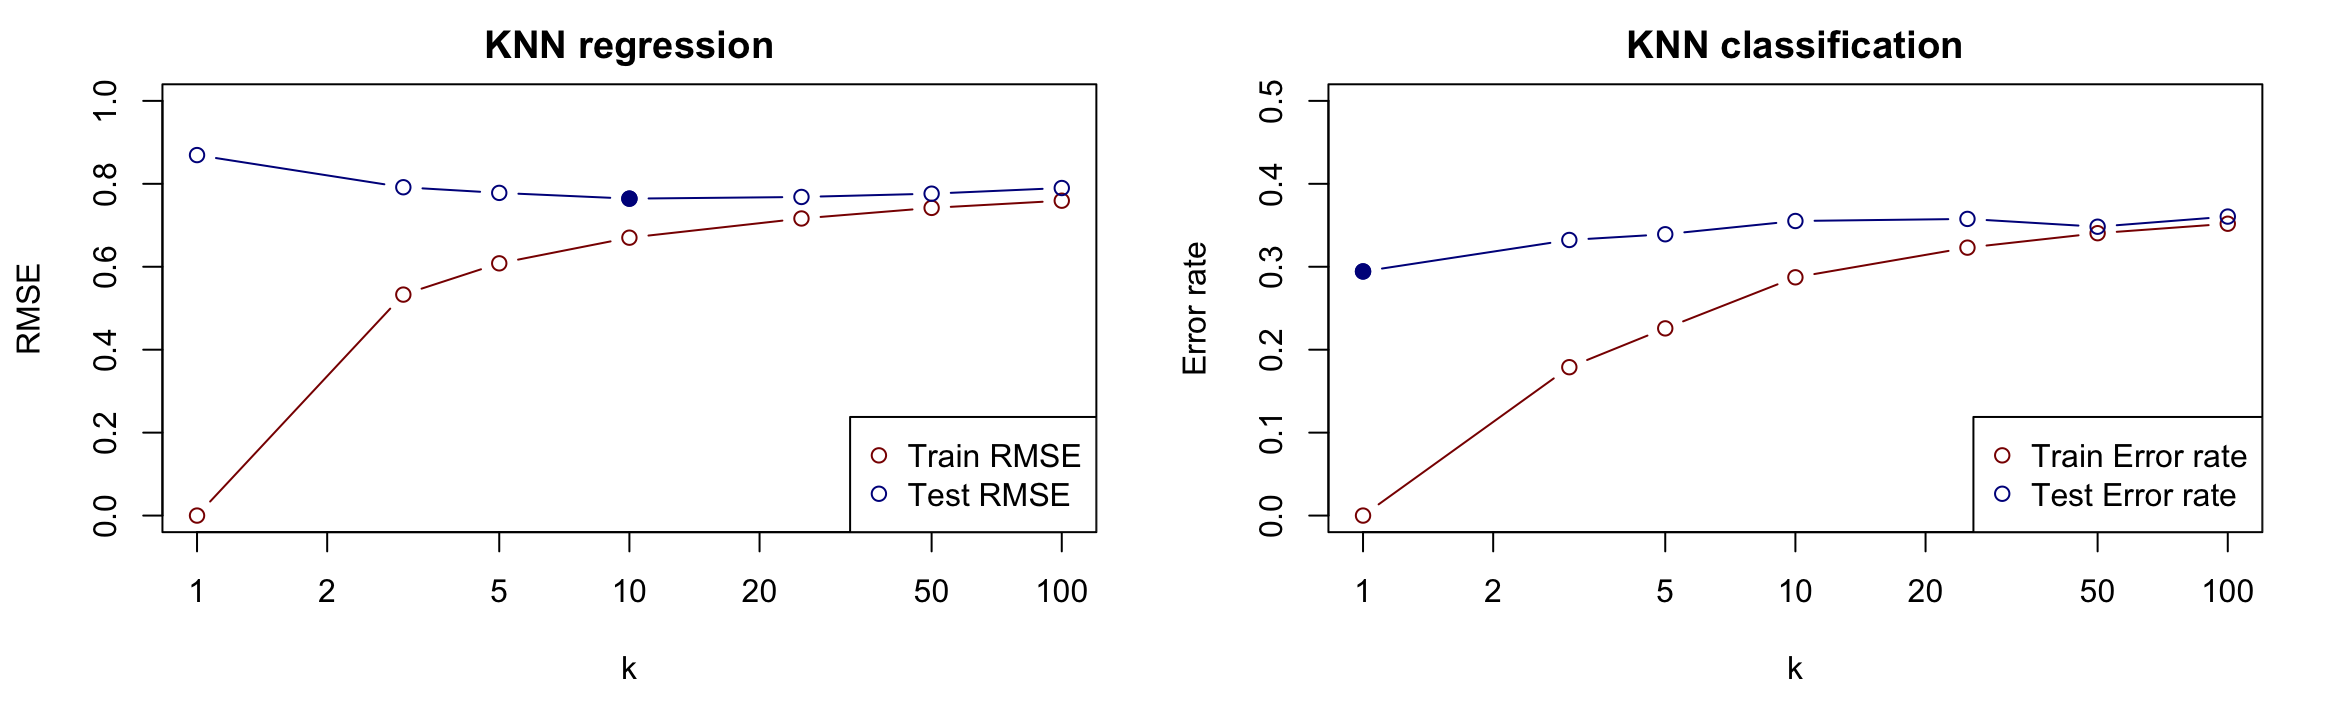
\includegraphics[scale=0.2]{knn.png}
    \caption{The performance of KNN  vs the value of K}
    \label{knn}
    
\end{figure}
As depicted in Figure \ref{knn} the lowest test RMSE for regression happens at $k=10$ with the $RMSE = 0.76$. and for the classification with two classes of high quality and low quality the minimum test error rate takes place at $k=1$ with the error rate of $29\%$.

\subsection{2.4  Tree based Methods}
Tree based methods are some supervised learning algorithms that are mostly used for regression and classification. These methods are easy to interpret and competitive with other classification methods. In this section, we discuss four of these methods including decision trees, bagging, random forest and boosting. The data used in these algorithms is the original data without outliers.
\subsubsection{2.4.1  Decision Trees}
Decision Tree uses the if-then rule to classify and also predict the variables, and enables us to present the decisions virtually. The team applied the decision tree method to the data with two-level quality response and provide the Figure \ref{Tree}. The tree has $9$ internal nodes and $10$ terminal nodes and shows the frequency of the observations in each terminal node. We can observe the most important feature in determining the quality of red wine is alcohol which stands at the top of the tree. Furthermore, tree has same number of terminal nodes for Low and High quality.
\begin{figure}[H]
    \centering
    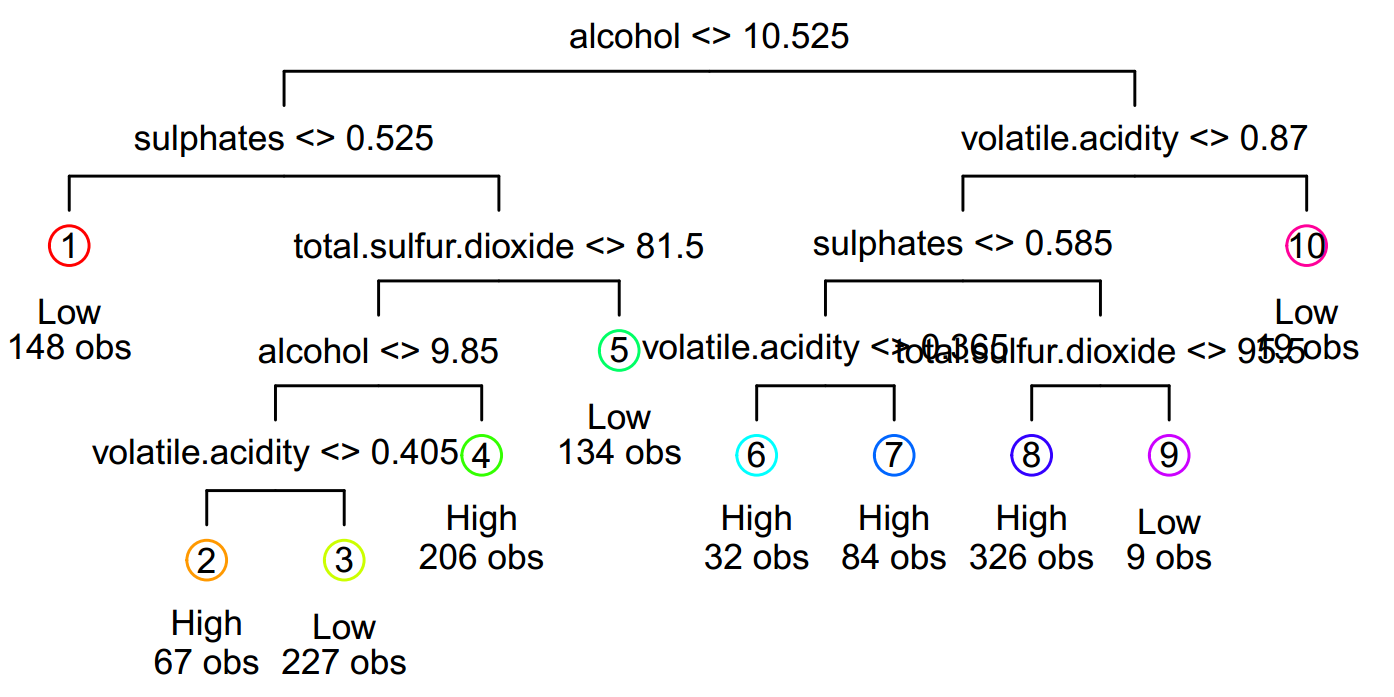
\includegraphics[scale=0.55]{Tree-Method.PNG}
    \caption{Decision Tree}
    \label{Tree}
\end{figure}
\subsubsection{2.4.2  Bagging and Random Forest Models}

Bagging is a technique to create many decision trees while ensuring their variety with random sampling. In fact, the method reduces the high variance we may counter in the decision tree method. We implement this method along with random forest. For the bagging part, we used all the predictors and the results are as below.

\begin{figure}[H]
\begin{minipage}[]{.5\textwidth}
    \centering
    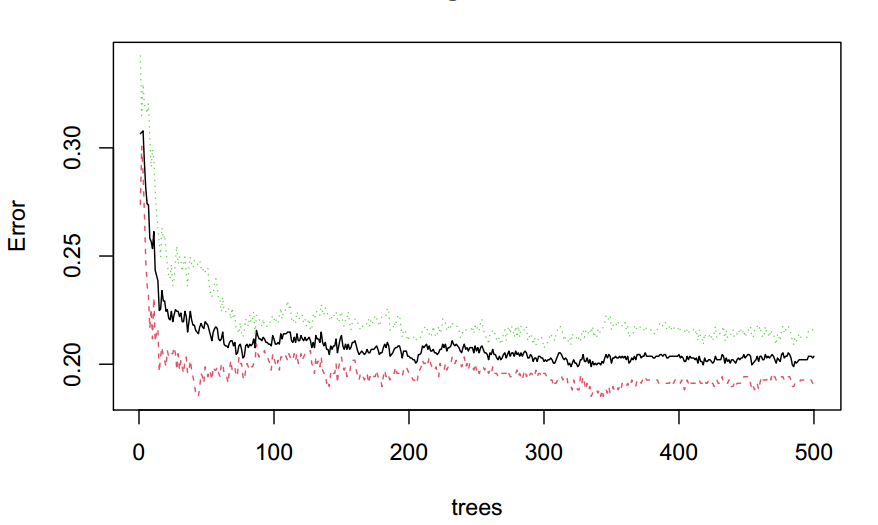
\includegraphics[scale=0.6]{Bagging1.PNG}
    \label{fig:Bagging1}
    \caption{Tree vs Error for bagging model}
\end{minipage}
\hspace{0.5cm}
\begin{minipage}[]{.5\textwidth}
    \centering
    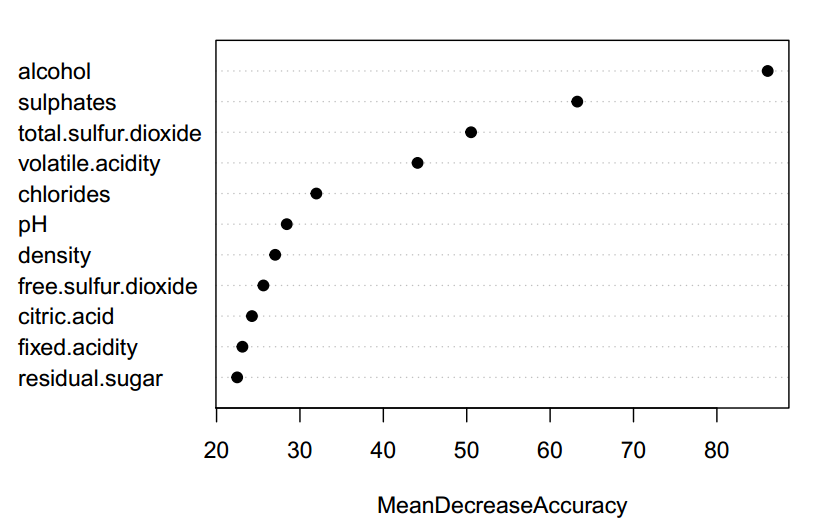
\includegraphics[scale=0.6]{Bagging2.PNG}
    \label{fig:Bagging2}
    \caption{Important variables according to bagging}
\end{minipage}
\end{figure}


%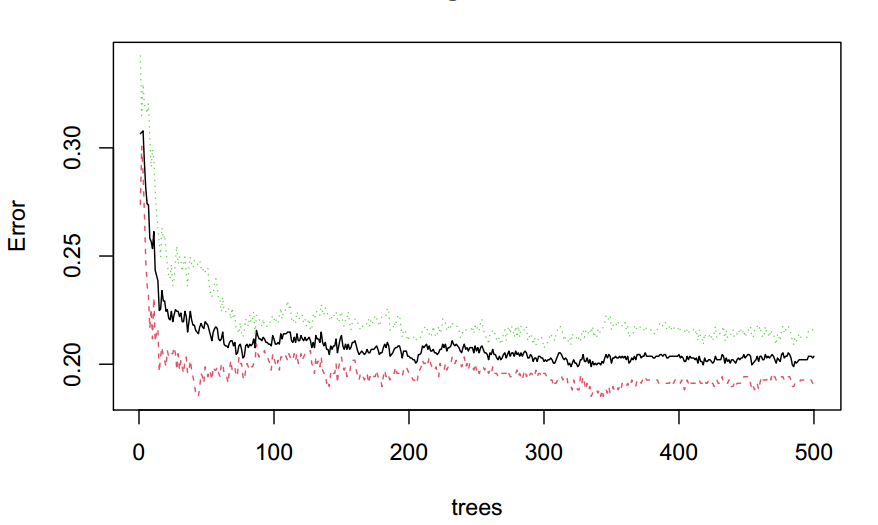
\includegraphics[scale=0.55]{Bagging1.PNG}
%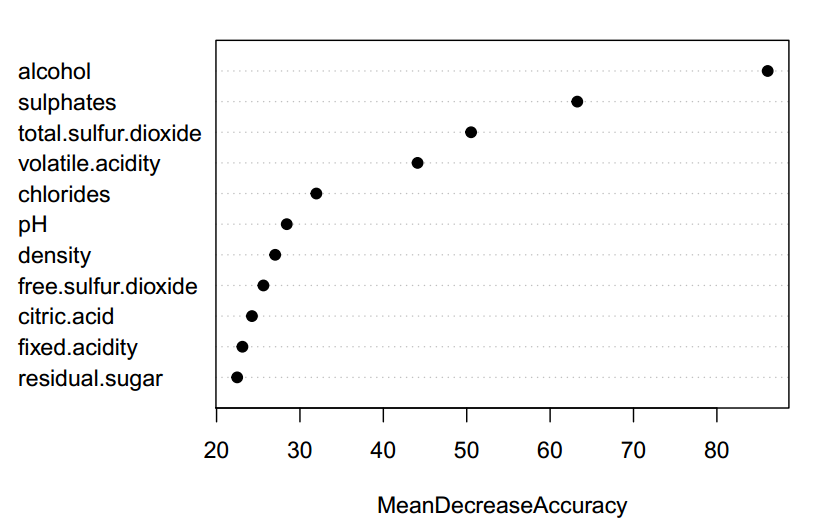
\includegraphics[scale=0.55]{Bagging2.PNG}
\
\\We can observe that four important features are "alcohol", "sulphates", "total.sulfur.dioxide" and "volatile.acidity". It seems that the error is almost constant after 250 trees. We will present the test errors for the methods in the results section.\\
We performed a cross-validation to figure out the best number of predictors in random forest model. Although there is not a significant difference in the accuracy of the models, $3$ predictor model shows better results, so we set $mtry=3$. We have almost the same important predictors except density comparing with bagging. We also set the number of trees equal to $10000$ but there is not much difference after less that $1000$ trees.

\begin{figure}[H]
\begin{minipage}[]{.4\textwidth}
    \centering
    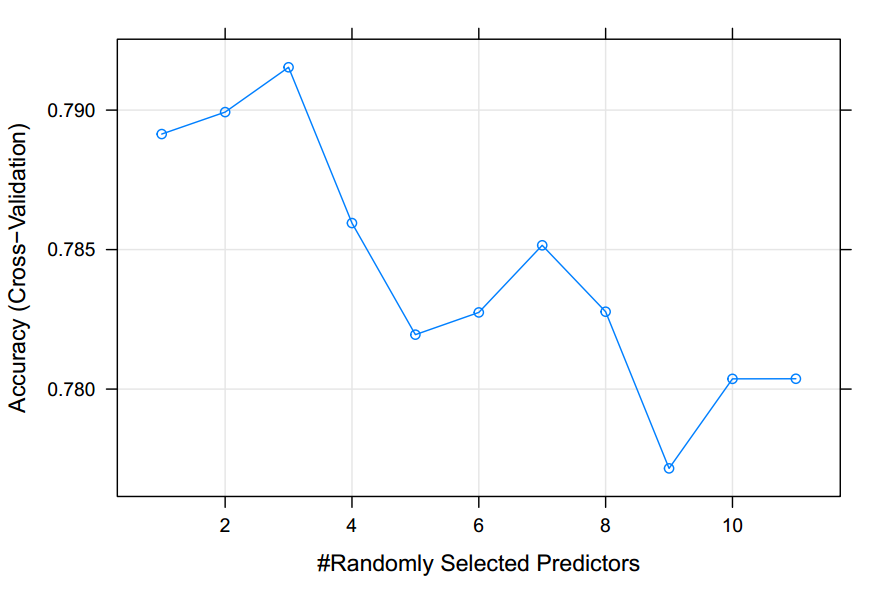
\includegraphics[scale=0.5]{RandomForest1.PNG}
        \caption{Accuracy vs number of predictors} 

   
    \label{fig:RF1}
\end{minipage}
\hspace{0.5cm}
\begin{minipage}[]{.6\textwidth}
    \centering
    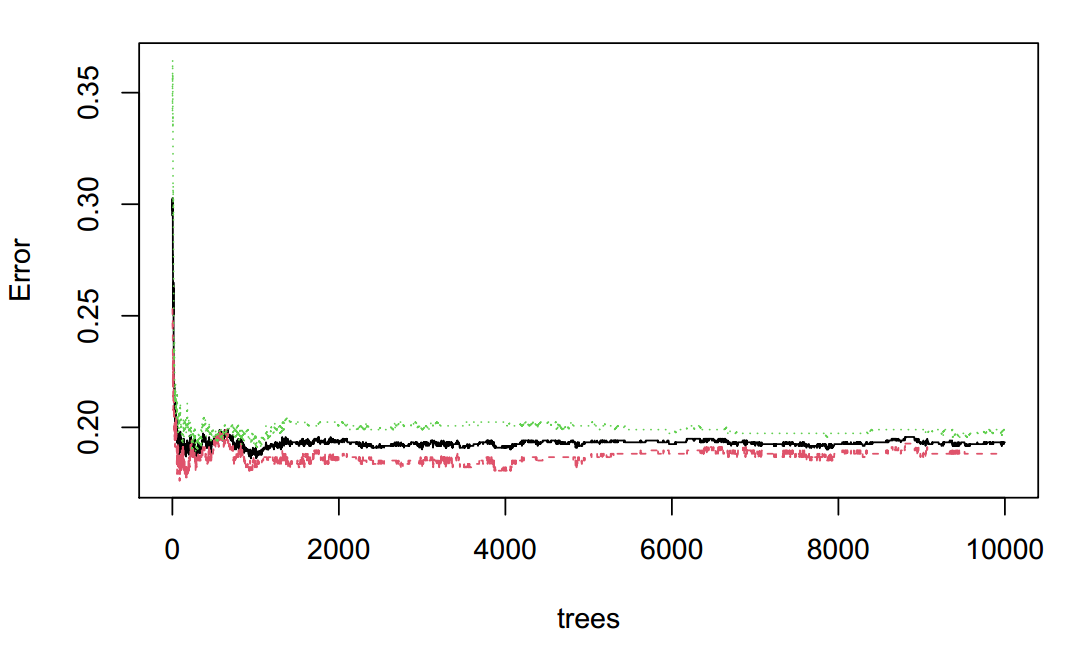
\includegraphics[scale=0.45]{RandomForest2.PNG}
    \caption{Trees vs Error for random forest}
    \label{fig:RF2}
\end{minipage}
\end{figure}


\begin{figure}[H]
    \centering
    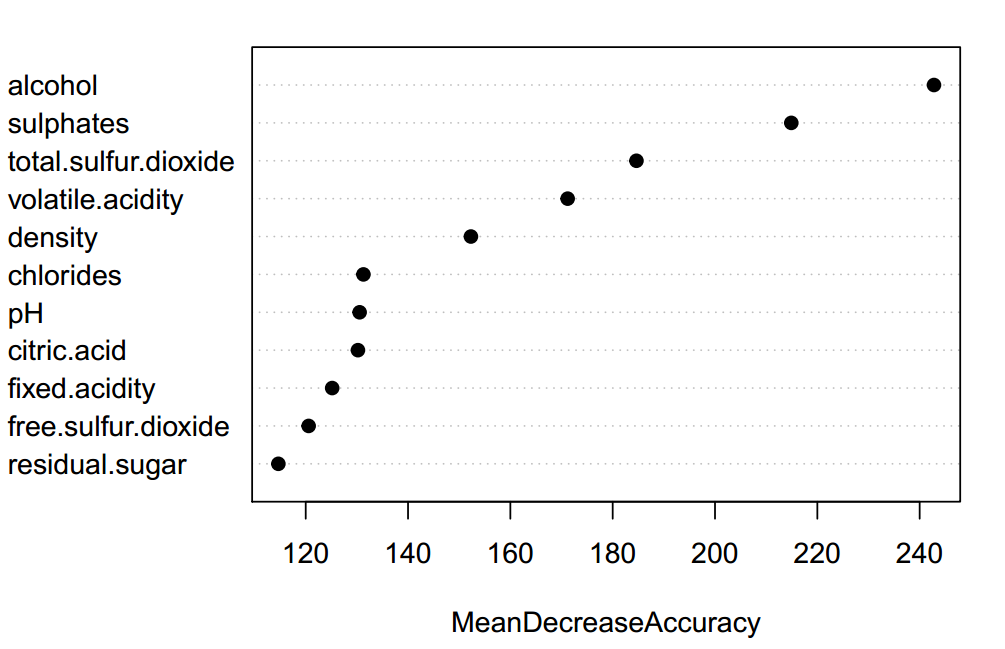
\includegraphics[scale=0.65]{RandomForest3.PNG}
    \caption{Important factors based on random forest}
    \label{fig:RF3}
\end{figure}

\subsubsection{2.4.3  Boosting}
Another powerful and accurate method for classification is boosting which creates consecutive small trees. That is, the method fit tree based on the residuals to ensure the balance between the over-fitting and variance. We also explored the best shrinkage level with cross validation on the train set, and set it as the shrinkage level in our analysis, but in fact it does not guarantee better performance on the test set. Figure \ref{Boosting} shows the importance of the variables based on this model.
\begin{figure}[H]
    \centering
    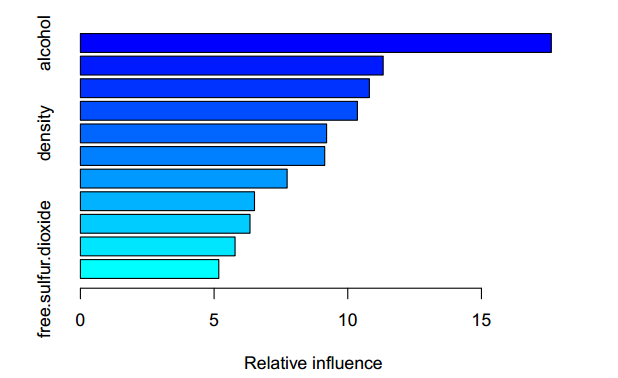
\includegraphics[scale=0.6]{Boosting.PNG}
    \caption{Importance of the variables with boosting}
    \label{Boosting}
\end{figure}
To summarize, the tree based models have competitive performances except the decision tree. Bagging and random forest perform very close and in some cases bagging works better but its average test error is a little bit worse than random forest. Although, decision tree has the worst performance among the methods, it is one of the interpretable models along with KNN.
\subsection{2.5  Support Vector Machines}
Support Vector Machines attempt to separate the data through use of a hyperplane in the same dimension as the data. SVMs with Linear, Polynomial, and Radial kernels were fit to the training set. In a simulation in which new train and test sets were formed each time, the test error was consistently lower for the Radial kernel. Figure \ref{SVM Test Error Simulation} only includes Linear and Radial kernels as the Polynomial kernel improved on the test error for a  Linear kernel by a small amount relative to the decrease in test error for Radial kernels.
\begin{figure}[H]
    \centering
    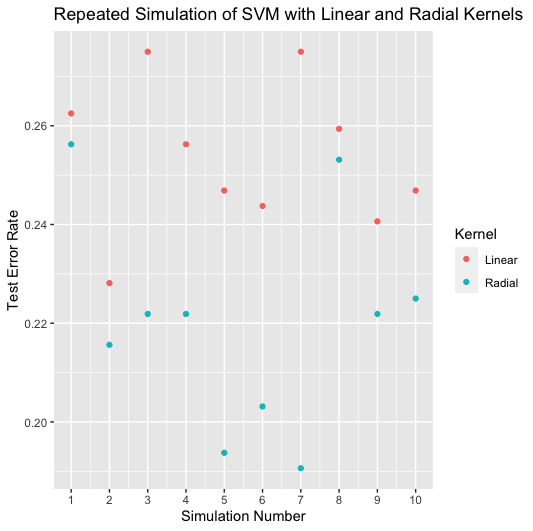
\includegraphics[scale=0.6]{Error_Sim_Plot.png}
    \caption{Simulated Test Error rates by Kernel}
    \label{SVM Test Error Simulation}
\end{figure}
For each iteration of this simulation (and for the model used to compare to other methods), the parameter associated with penalizing the SVM for training misclassification was fit using grid search cross validation for values: (0.001, 0.01, 0.1, 1, 5, 10, 100) for both Radial and Linear kernels. For Radial kernels, the additional parameter of gamma was fit using grid search cross validation on values: (0.5, 1, 2, 3, 4). 

On average, the Radial kernel decreased test error by about 3\% compared to an SVM using a Linear kernel on the same data. This suggests that we need a little more complicated surface than a hyperplane to capture the separation of our data into high and low quality. In practice, this may be an unfortunate result since the Radial kernel SVM is a little more costly to fit for data in higher dimensions. If the dataset were much larger with more variables, we would probably have selected the Linear kernel SVM. However, with this dataset, we selected the Radial Kernel SVM to report in the Results section. 

The group considered the removal of variables as well. When the pair of kernels were trained on the reduced model, the resulting test errors were significantly higher than that of using all 11 features. Because there are relatively few variables, the models fit are not likely to suffer due to dimensionality. It was therefore concluded that we should use all variables on the SVM classification.  

\section{3   Results}
In the previous sections several classification and regression methods  were explored. The models and their hyper parameters were tuned so the best performance of each model were obtained. In this section the error rate of different classification methods are compared in multiple simulations. The setup for all the methods are similar in terms of the split of training and testing sets. Additionally the outlier data points were removed for the tree based methods.
\begin{figure}[H]
    \centering
    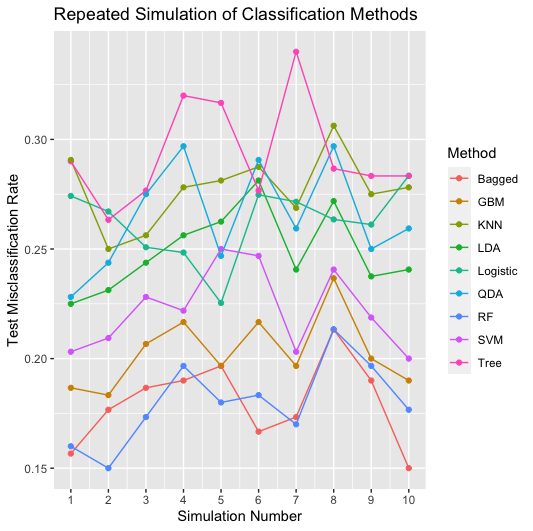
\includegraphics[scale=0.6]{finalErrorPlots.png}
    \caption{Error rates of methods in 10 simulations}
    \label{sims}
\end{figure}
\begin{figure}[H]
    \centering
    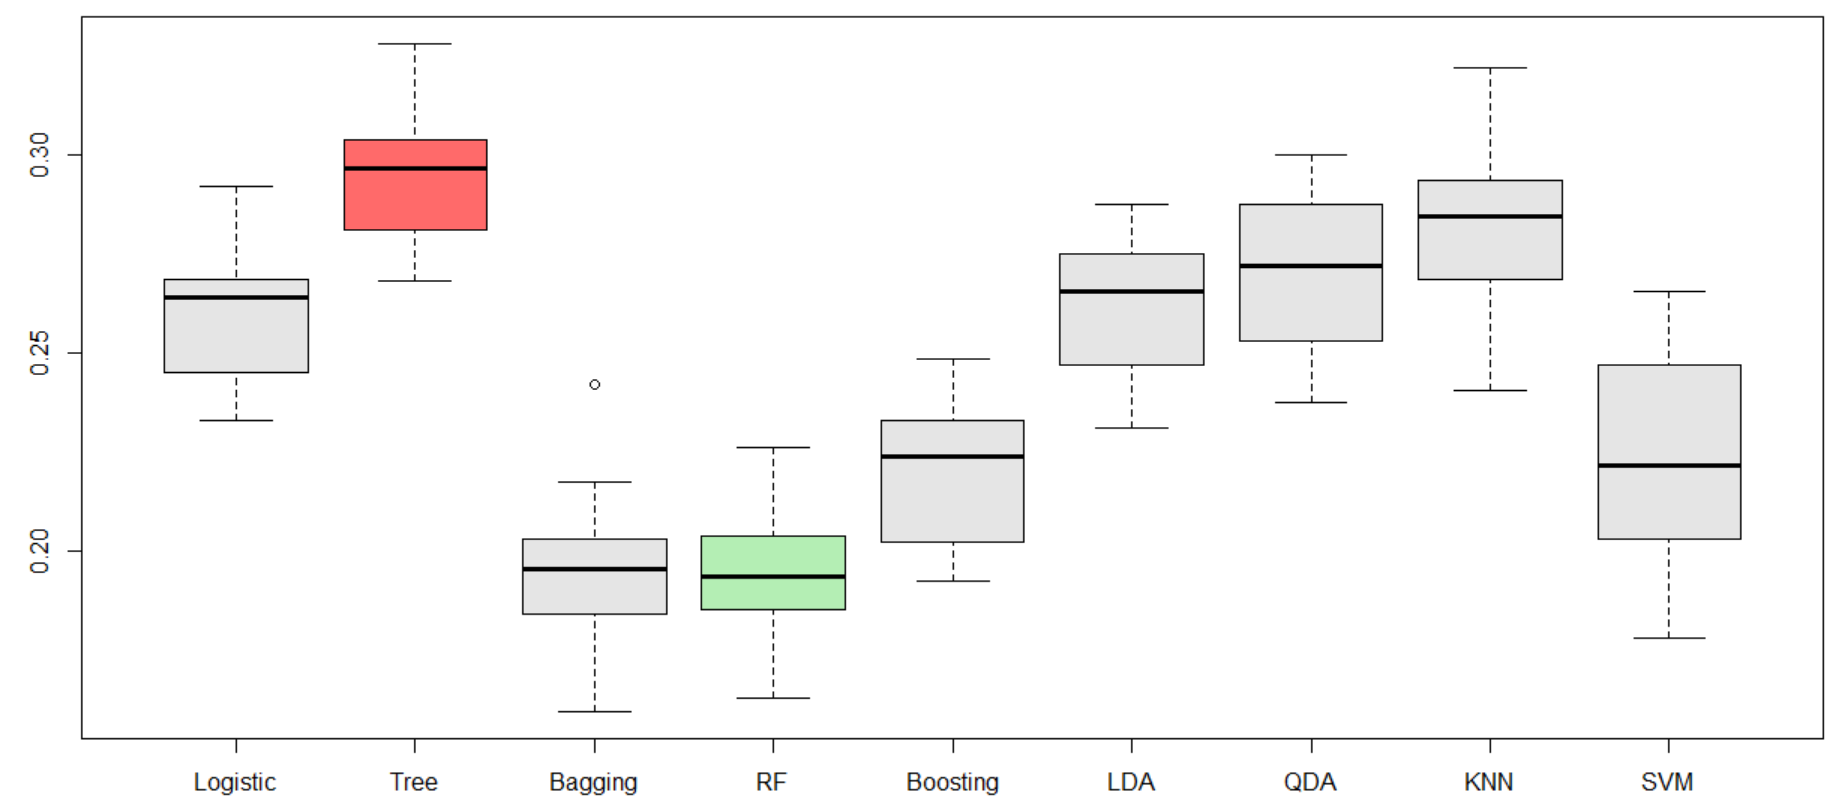
\includegraphics[scale=0.4]{Boxplot2.PNG}
    \caption{Error rates of methods}
    \label{sims2}
\end{figure}

\vspace{0.5cm}
As shown in Figure \ref{sims} the error rates for each method is plotted in the simulations. It is clear the bagged trees and random forest consistently come first and therefore are the most reliable models for the wine classification. On the other side of the spectrum KNN and decision tree tend to perform poorly. As discussed in section 2.3 the best value for K turned out to be one, which means the model is not learning complex relations and is predicting based on just local data. The same line of argument is true for decision tree.

\begin{table}[H]
    \centering
    \begin{tabular}{c|c|| c|c}
    \hline
        Model & Error rate & Model & Error rate\\
        \hline
        \hline
        Logistic Regression & 0.260 &KNN & 0.285\\
        LDA & 0.262 & QDA & 0.270 \\
         \cellcolor{red!30}Decision Tree &  \cellcolor{red!30}0.295 & Bagged Trees &0.196\\
        GBM & 0.220 &\cellcolor{green!30} Random Forest &\cellcolor{green!30} 0.194\\
        SVM& 0.222 & & \\
         \hline
    \end{tabular}
    \caption{Average classification error rates of the methods}
    \label{summary}
\end{table}

The summary of classification error rates are shown in Table \ref{summary}. Among all the methods random forest achieves the best accuracy with the error rate of $19.4 \%$ and the worst performance belongs to decision tree with error rate of $29.5 \%$. It is worth mentioning that even though SVM is one of the better performers it is the most computationally expensive method. 

\section{4  Conclusion}
In this project the red wine data was analysed via several methods, namely, logistic regression, LDA, QDA, KNN, tree based methods and SVM. The data was investigated with respect to the histogram of different variables and quality. The wine samples were labeled as "High" quality and "Low" quality forming a two class data set.  Additionally, variable selection was performed on the data in order to reduce the dimension of data set. The outlier data points were recognized in order to exclude from tree methods training. All the methods were thoroughly investigated and fine tuned. The models were compared with respect to test set error rates and random forest and bagged trees tended to be more accurate with better performance in terms of training time, while decision tree and KNN are least accurate.

\newpage
\section{5  Appendix}
\subfile{AppendixFiles/Appendix}


\end{document}
